\section{Método da Diferenciação dos Polinômios de Interpolação de Newton}

\begin{enumerar}

\item O polinômio de interpolação \textit{forward} de \textit{Newton} é:

\begin{equation}
 \label{cap3:sec3:eq1}
 g\,(x) = g\,(x_k + s\,h) = \sum_{n=0}^N \, \left(s \atop n\right) \, \Delta^n \, f_k
\end{equation}

\begin{figure}[htb]
 \centering
 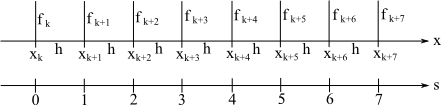
\includegraphics[scale=1.0]{capitulos/capitulo3/figuras/met_dif_pol_int_new1.png}
 \caption{?}
 \label{fig:met_dif_pol_int_new1}
\end{figure}

\begin{equation}
 \label{cap3:sec3:eq2}
 s = \frac{x - x_k}{h}
\end{equation}

\begin{equation}
 \label{cap3:sec3:eq3}
 \left(s \atop n\right) = \frac{s!}{n!\,(s-n)!}
\end{equation}

\begin{equation}
 \label{cap3:sec3:eq4}
 \begin{array}{ll}
  g\,(x) & = g\,(x_k + s\,h) \vspace*{0.2cm} \\
         & = f_k + s\,\Delta\,f_k + \displaystyle \frac{1}{2} \, s\,(s-1)\,\Delta^2\,f_k + \frac{1}{6} \, s\,(s-1)\,(s-2)\,\Delta^3\,f_k \vspace*{0.2cm} \\
         & + \displaystyle \frac{1}{24}\,s\,(s-1)\,(s-2)\,(s-3)\,\Delta^4\,f_k + \ldots + \left(s \atop n\right) \, \Delta^N \, f_k
 \end{array}
\end{equation}

\textbf{OBS:}

O polinômio \esp{g\,(x) = g\,(x_k + s\,h) = \sum_{n=0}^N \, \left( s \atop n \right) \, \Delta^n \, f_k} tem ordem $n$ e passa por $n+1$ pontos amostrais.

\item Para $n = 2 \Rightarrow$ 3 pontos

\begin{equation}
 \label{cap3:sec3:eq5}
 g\,(x) = f_k + s\,\Delta\,f_k + \frac{1}{2}\,s\,(s-1)\,\Delta^2\,f_k
\end{equation}

\begin{equation}
 \label{cap3:sec3:eq6}
 g'\,(x) = \frac{1}{h} \, \left[ \Delta\,f_k + \frac{1}{2}\,(2\,s-1)\,\Delta^2\,f_k \right]
\end{equation}

Para $s = 0$, $1$ e $2$:

\begin{equation}
 \label{cap3:sec3:eq7}
 g'\,(x_k) = \frac{1}{2\,h} \, \left[ 2\,\Delta\,f_k - \Delta^2\,f_k \right] = \frac{1}{2\,h} \, \left[ -f_{k+2} + 4\,f_{k+1} - 3\,f_k \right]
\end{equation}

\begin{equation}
 \label{cap3:sec3:eq8}
 g'\,(x_{k+1}) = \frac{1}{2\,h} \, \left[ 2\,\Delta\,f_k + \Delta^2\,f_k \right] = \frac{1}{2\,h} \, \left[ f_{k+2} - f_k \right]
\end{equation}

\begin{equation}
 \label{cap3:sec3:eq9}
 g'\,(x_{k+2}) = \frac{1}{2\,h} \, \left[ 2\,\Delta\,f_k + 3\,\Delta^2\,f_k \right] = \frac{1}{2\,h} \, \left[ 3\,f_{k+2} - 4\,f_{k+1} + f_k \right]
\end{equation}

$k = i$ (\textit{Forward} 3 pontos)

\begin{equation}
 \label{cap3:sec3:eq10}
 g'\,(x_i) = \frac{1}{2\,h} \, \left[ 2\,\Delta\,f_i - \Delta^2\,f_i \right] = \frac{1}{2\,h} \, \left[ -f_{i+2} + 4\,f_{i+1} - 3\,f_i \right]
\end{equation}

$k + 1 = i$ (Centrada 3 pontos)

\begin{equation}
 \label{cap3:sec3:eq11}
 g'\,(x_i) = \frac{1}{2\,h} \, \left[ 2\,\Delta\,f_{i-1} + \Delta^2\,f_{i-1} \right] = \frac{1}{2\,h} \, \left[ f_{i+1} - f_{i-1} \right]
\end{equation}

$k + 2 = i$ (\textit{Backward} 3 pontos)

\begin{equation}
 \label{cap3:sec3:eq12}
 g'\,(x_i) = \frac{1}{2\,h} \, \left[ 2\,\Delta\,f_{i-2} + 3\,\Delta^2\,f_{i-2} \right] = \frac{1}{2\,h} \, \left[ 3\,f_i - 4\,f_{i-1} + f_{i-2} \right]
\end{equation}

\item Erro

Se tivermos mais um ponto amostral, o polinômio interpolante representa melhor a função interpolada. Assim, o erro do polinômio de \textit{Newton} é representado pelo termo que seria adicionado caso um ponto amostral a mais seja introduzido.

Se, por exemplo, aumentarmos de $n = 2$ para $n = 3$, o termo:

\begin{equation}
 \label{cap3:sec3:eq13}
 \frac{1}{6} \, s\,(s-1)\,(s-2) \, \Delta^3 f_k
\end{equation}

seria acrescido \`a  equa\'c\~ao (\ref{cap3:sec3:eq5}), e sua derivada seria

\begin{equation}
 \label{cap3:sec3:eq14}
 \frac{1}{6\,h} \, \left[ 3\,s^2 - 6\,s + 2 \right] \, \Delta^3 \, f_k
\end{equation}

Para

\begin{equation}
 \label{cap3:sec3:eq15}
 s = 0 \rightarrow \frac{1}{3\,h} \, \Delta^{3}f_{k} \qquad Forward
\end{equation}

\begin{equation}
 \label{cap3:sec3:eq16}
 s = 1 \rightarrow \frac{1}{6\,h} \, \Delta^{3}f_{k} \qquad Centrada
\end{equation}

\begin{equation}
 \label{cap3:sec3:eq17}
 s = 2 \rightarrow \frac{1}{3\,h} \, \Delta^{3}f_{k} \qquad Backward
\end{equation}

\end{enumerar}

\textbf{OBS:}

A e-enésima derivada de $g(x)$ de ordem $n$ é:

\begin{equation}
 \label{cap3:sec3:eq18}
 \frac{d^n}{dx^n} \, g\,(x) = \frac{1}{h^n} \, \Delta^n \, f_i
\end{equation}

Assim,

\begin{equation}
 \label{cap3:sec3:eq19}
 \Delta^n\,f_i \approx h^n \, f^{(n)}(x)
\end{equation}

Portanto, as expressões (\ref{cap3:sec3:eq15}) a (\ref{cap3:sec3:eq17}) ficam:
\[
 \displaystyle \frac{1}{3}\,h^{2}\,f'''_{k}\,, \mbox{ para } s = 0
\]

\[
 \displaystyle -\frac{1}{6}\,h^{2}\,f'''_{k}\,, \mbox{ para } s = 1
\]

\[
 \displaystyle \frac{1}{3}\,h^{2}\,f'''_{k}\,, \mbox{ para } s = 2
\]
